\chapter{Keil Software Development Tools}
\label{ch_keil_software}

The Keil MDK-ARM development tools are used for MCB1700 boards in our lab.
The tools include
\begin{itemize}
\item uVision5 IDE which combines the project manager, source code editor and program debugger into one environment; 
\item ARM compiler, assembler, linker and utilities;
\item ULINK USB-JTAG Adapter which allows you to debug the embedded programs running on the board.
\end{itemize}

The MDK-Lite is the evaluation version and does not require a license. 
It has a code size limit of 32KB, which is adequate for the lab projects.
The MDK-Lite version 5 is installed on all lab computers. 
If you want to install the software on your own computer. MDK 5.30 installation file is in Learn Lab/RTX Project section. The downloading link for the latest version is \url{https://www2.keil.com/mdk5/editions/lite}. 
%Appendix \ref{app_keil_install} gives detailed instruction.

%\section{Creating an Application in uVision5 IDE}
%\label{sec_uvision_app}
\section{Getting Started with uVision5 IDE}
To get started with the Keil IDE, the Getting Started with MDK Guide at
\url{https://www.keil.com/support/man/docs/mdk_gs/} 
is a good place to start. We will walk you through the IDE by developing
a simple HelloWorld application which displays Hello World through the UART0 and UART1
that are connected to the lab PC. Note the HelloWorld example uses polling on both UART0 and UART1 rather than interrupt. 

\section{Getting Starter Code from the GitHub}
The SE 350 lab starter github is at \url{https://github.com/yqh/SE350}. Let's first make a clone of this repository by using the following command:
\begin{lstlisting}[style=bash]
 git clone https://github.com/yqh/SE350.git 
\end{lstlisting}

\section{Start the Keil uVision5 IDE}
The Keil uVision5 IDE shortcut should be accessible from the start menu on school computers. If not, then navigate to \verb+C:\Software\Keil_v5\UV4+ folder and double click the {\bf UV4.exe} to bring up the IDE (see Figure \ref{fig_ide_uv5_location}). 
\begin{figure}[ht!]
\centerline{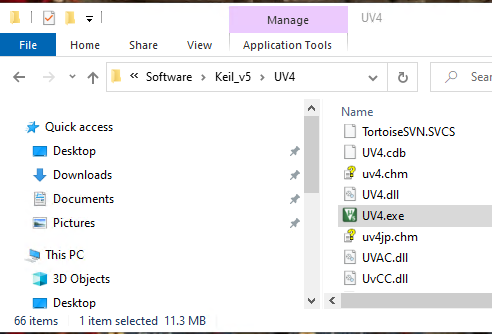
\includegraphics[width=4in]{figure/uv5/IDE_uv5_location}}
\caption{Keil IDE: Create a New Project} 
\label{fig_ide_uv5_location}
\end{figure}

\section{Create a New uVision5 Project}
\begin{enumerate}
    \item Create a directory named ``HelloWorld" on your computer. The folder path name should not contain spaces on Nexus computers.
    \item Create a sub-directory ``src'' under the ``HelloWorld'' directory. This sub-folder is where we want to put our source code of the project. 
    \item Copy the following files to ``src" folder:
    \begin{itemize}
        \item \verb+manual_code/util/printf_uart/uart_def.h+
        \item \verb+manual_code/util/printf_uart/uart_polling.h+
        \item \verb+manual_code/util/printf_uart/uart_polling.c+
    \end{itemize}
    \item Create a new uVision project.\\ 
Open the file explorer and navigate to \verb+C:\Software\Keil_v5\UV4+. Double click the \verb+UV4.exe+ program to start the IDE.
    \begin{itemize}
        \item Click Project $\rightarrow$ New uVision Project (See Figure \ref{fig_ide_new_proj}). \par
          \begin{minipage}[t]{\linewidth}
            \centering
            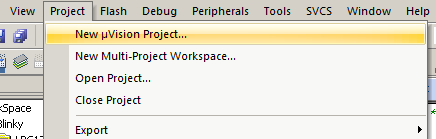
\includegraphics[width=4in]{figure/IDE_new_proj}
            \captionof{figure}{Keil IDE: Create a New Project} 
            \label{fig_ide_new_proj}
           \end{minipage}
        \item Select NXP $\rightarrow$ LPC1700 Series $\rightarrow$ LPC176x $\rightarrow$ LPC1768 (See Figure \ref{fig_ide_nxp_lpc1768}). \par

          \begin{minipage}[t]{\linewidth}
            \centering
            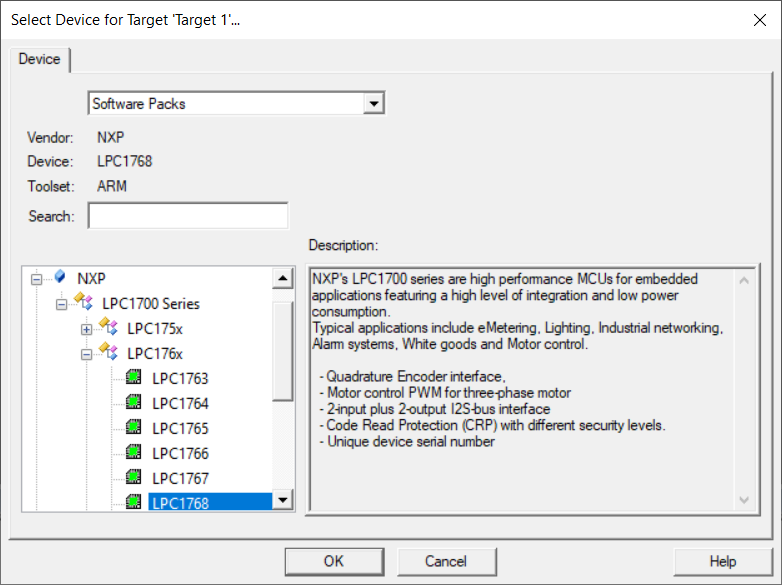
\includegraphics[width=4in]{figure/uv5/IDE_NXP_LPC1768}
            \captionof{figure}{Keil IDE: Choose MCU}
            \label{fig_ide_nxp_lpc1768}
          \end{minipage}
            
        \item Select CMSIS $\rightarrow$ CORE and Device $\rightarrow$ Startup (See Figure \ref{fig_ide_runtime_env}). \par 
          \begin{minipage}{\linewidth}
            \centering
            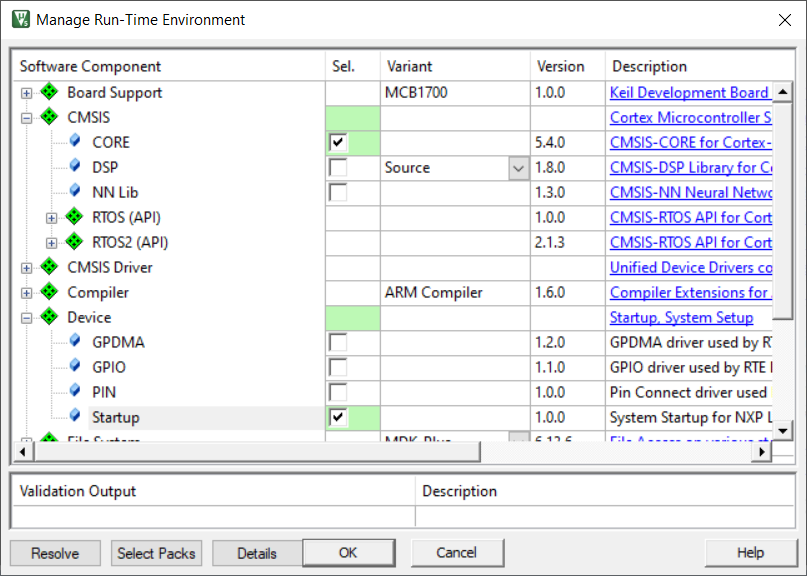
\includegraphics[width=4in]{figure/uv5/IDE_Runtime_Env}
            \captionof{figure}{Keil IDE: Manage Run-time Environment}
            \label{fig_ide_runtime_env}
          \end{minipage}
    \end{itemize}
\end{enumerate}

\section{Managing Project Components}
You just finished creating a new project. One the left side of the IDE is the Project window. Expand all objects. You will see the default project setup as shown in Figure \ref{fig_ide_default_proj}.


  \begin{minipage}{\linewidth}
    \centering
    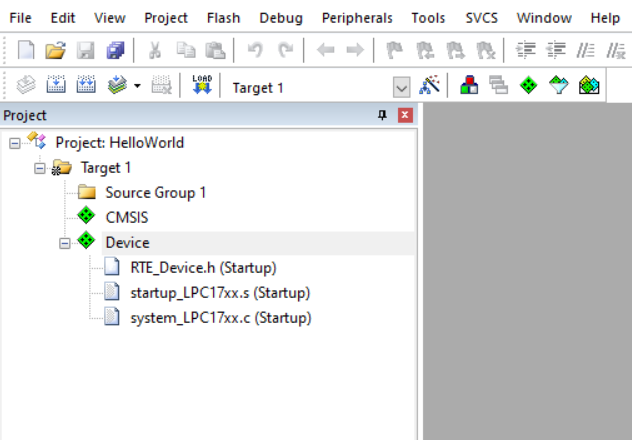
\includegraphics[width=4in]{figure/uv5/IDE_default_proj}
    \captionof{figure}{Keil IDE: A default new project} 
    \label{fig_ide_default_proj}
  \end{minipage}

\begin{enumerate}
  \item{Rename the Target}\\ 
    The ``Target 1``is the default name of the project build target and you can rename it.
    Select the target name to highlight it and then long press the left button of
    the mouse to make the target name editable.
    Input a new target name, say ``HelloWorld SIM".   

  \item{Rename the Source Group} \\
    The IDE allows you to group source files to different groups to better manage the source code.
    By default ``Source Group 1`` is created and it contains no file.
    Let's rename the source group to ``System Code"
    \footnote{To rename a source group, select the source group to highlight it and long press the left mouse button to make the name editable.}. 

  \item{Add a New Source Group} \\
  We can also add new source group in our project.
  Select the HelloWorld SIM item and right click to bring up the context window and
  select ``Add Group...'' (See Figure \ref{fig_ide_add_group}).\par 

    \begin{minipage}{\linewidth}
      \centering
      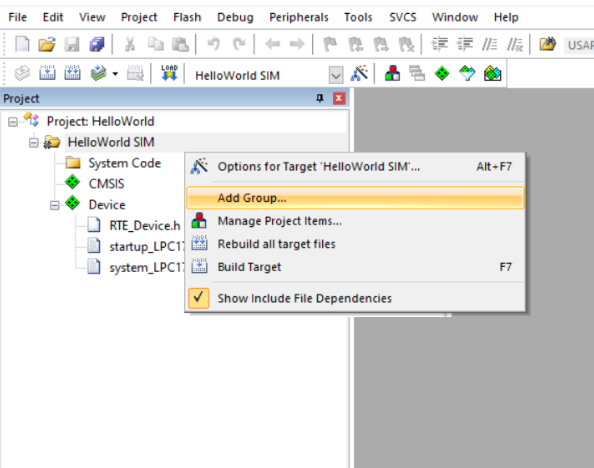
\includegraphics[width=4in]{figure/uv5/IDE_add_group}
      \captionof{figure}{Keil IDE: Add Group} 
      \label{fig_ide_add_group}
    \end{minipage}

    A new source group named ``New Group'' is added to the project.
    Let's rename it to ``User Code``. 
    Your project will now look like Figure \ref{fig_ide_proj_new_group}. \par

    \begin{minipage}{\linewidth}
      \centering
      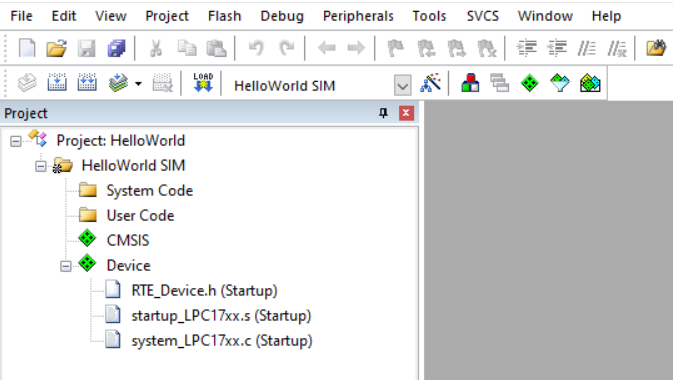
\includegraphics[width=4in]{figure/uv5/IDE_proj_new_group}
      \captionof{figure}{Keil IDE: Updated Project Profile} 
      \label{fig_ide_proj_new_group}
    \end{minipage}

  \item{Add Source Code to a Source Group} \\
    Let's add \verb+uart_polling.c+ to ``System Code" group by double clicking the source group and
    choose the file from the file window.
    Double clicking the file name will add the file to the source group.
    Or you can select the file and click the ``Add" button at the lower right corner of the window 
    (See Figure \ref{fig_ide_add_src}). \par

    \begin{minipage}{\linewidth}
      \centering
      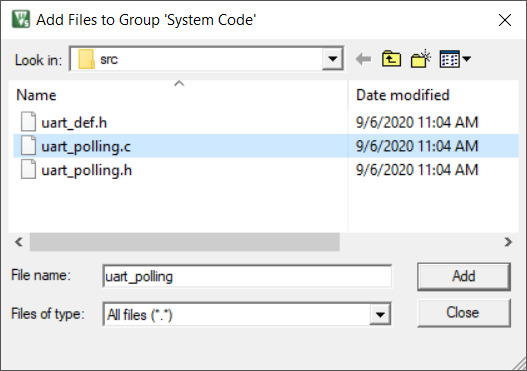
\includegraphics[width=3.5in]{figure/uv5/IDE_add_src}
      \captionof{figure}{Keil IDE: Add Source File to Source Group} 
      \label{fig_ide_add_src}
    \end{minipage}

    Your project will now look like Figure \ref{fig_ide_proj_pre_final}. \par
    \begin{minipage}{\linewidth}
      \centering
      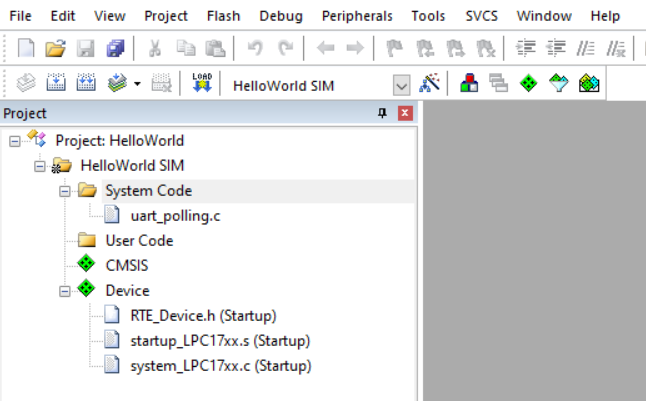
\includegraphics[width=4in]{figure/uv5/IDE_proj_pre_final}
      \captionof{figure}{Keil IDE: Updated Project Profile} 
      \label{fig_ide_proj_pre_final}
    \end{minipage}
 
  \item{Create a new source file} \\
   The project does not have a main function yet. We now create a new file by
   selecting File $\rightarrow$ New (See Figure \ref{fig_ide_new_file}). \par 

    \begin{minipage}{\linewidth}
      \centering
      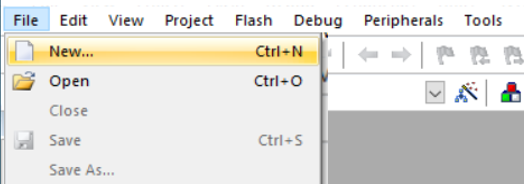
\includegraphics[width=4in]{figure/uv5/IDE_New_File}
      \captionof{figure}{Keil IDE: Create New File} 
      \label{fig_ide_new_file}
    \end{minipage}

    Before typing anything to the file, save the file and name it ``main.c". 
    Add main.c to the ``Source Code" group. Type the source code as shown in Figure \ref{fig_ide_proj_final}.
    Your final project would look like the screen shot in Figure \ref{fig_ide_proj_final}. \par

    \begin{minipage}{\linewidth}
      \centering
      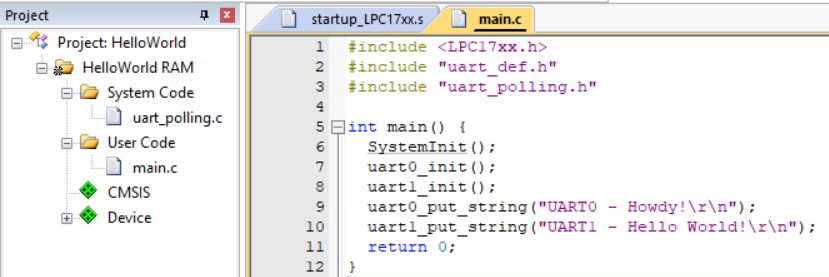
\includegraphics[width=4in]{figure/uv5/IDE_proj_final}
      \captionof{figure}{Keil IDE: Final Project Setting} 
      \label{fig_ide_proj_final}
    \end{minipage}

\end{enumerate}

\section{Build the Project Target}
\label{sec_target_configuration}
To build a target, the main work is to configure the target options.

\subsection{Configure Target Options}
\label{sec_target_option}
Most of the default settings of the target options are good. There are a few options that we need to modify.
  \begin{enumerate}
    \item Bring up the target option configuration window by pressing the target options button (See Figure \ref{fig_ide_target_options}). \par 

      \begin{minipage}{\linewidth}
        \centering
        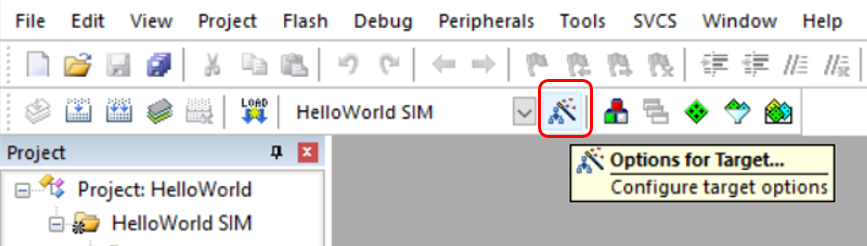
\includegraphics[width=4in]{figure/uv5/IDE_target_options}
        \captionof{figure}{Keil IDE: Target Options Configuration } 
        \label{fig_ide_target_options}
      \end{minipage}

    \item Configure the Target tab as shown in Figure \ref{fig_ide_opt_target_tab}.
      We want to use the default version 5 arm compiler.
      We also want remove the IRAM2 from the default setting. \par 

          \begin{minipage}{\linewidth}
            \centering
            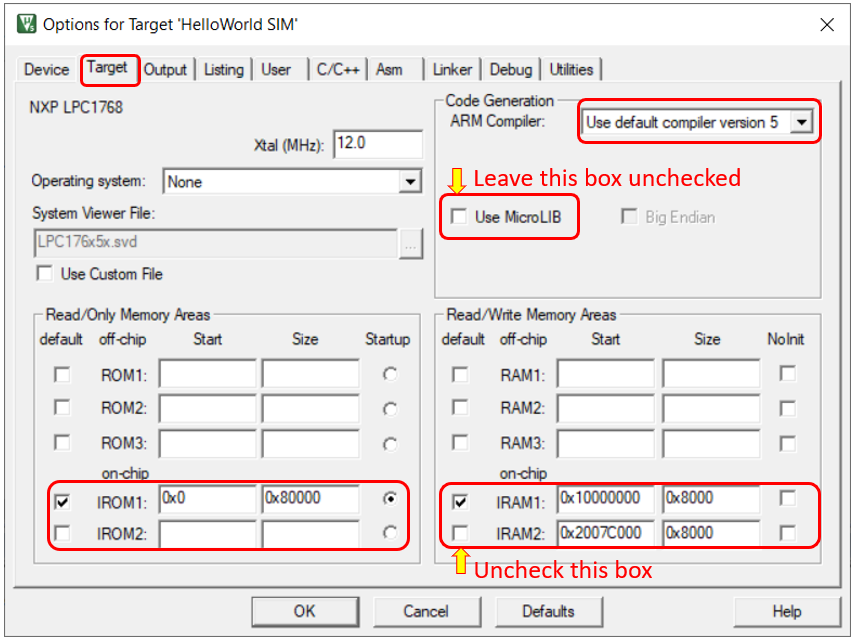
\includegraphics[width=4in]{figure/uv5/IDE_opt_target_tab}
            \captionof{figure}{Keil IDE: Target Options Target Tab Configuration } 
            \label{fig_ide_opt_target_tab}
          \end{minipage}

    \item Configure the C/C++ tab as shown in Figure \ref{fig_ide_opt_compiler_tab}.
      We do not need c99 for this example. So we leave it unchecked. \par

      \begin{minipage}{\linewidth}
        \centering
        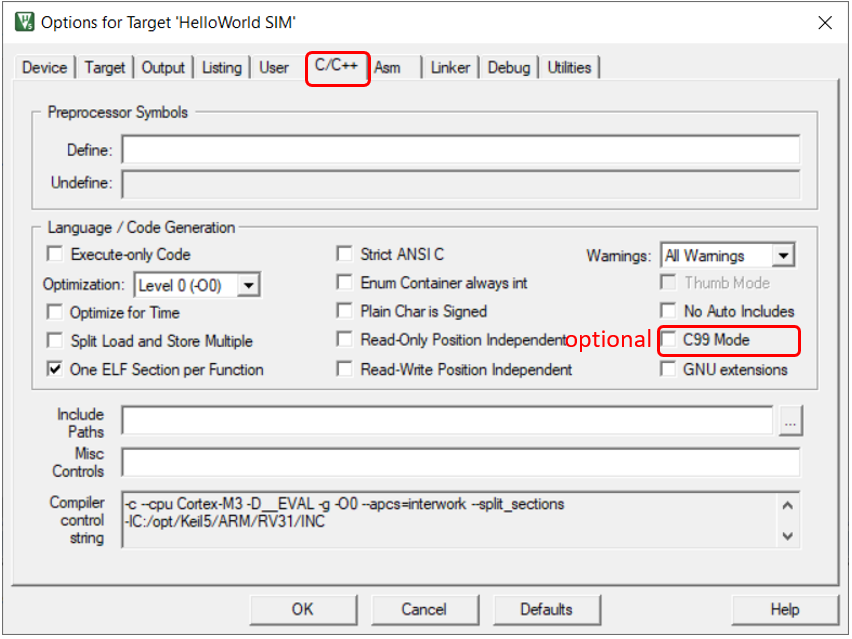
\includegraphics[width=4in]{figure/uv5/IDE_opt_compiler_tab}
        \captionof{figure}{Keil IDE: Target Options C/C++ Tab Configuration } 
        \label{fig_ide_opt_compiler_tab}
      \end{minipage}

    \item Configure the Linker tab as shown in Figure \ref{fig_ide_opt_linker_tab}.
      This is to instruct the linker to use the memory layout from the Target tab setting instead of the default memory layout.

      \begin{minipage}{\linewidth}
        \centering
        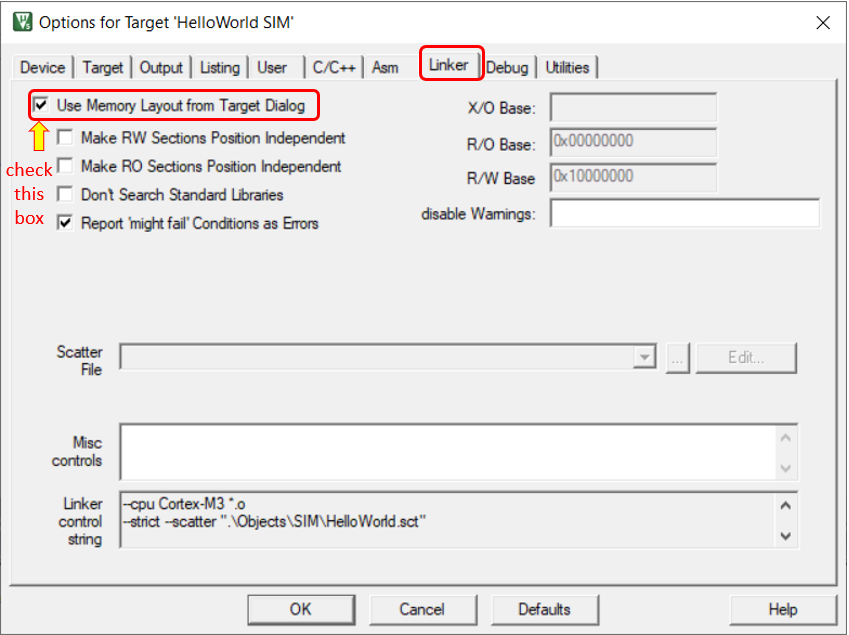
\includegraphics[width=4in]{figure/uv5/IDE_opt_linker_tab}
        \captionof{figure}{Keil IDE: Target Options Linker Tab Configuration } 
        \label{fig_ide_opt_linker_tab}
      \end{minipage}

  \end{enumerate}

  \subsection{Build the Target}
    To build the target, click the ``Build" button (see Figure \ref{fig_ide_build_button}). \par

    \begin{minipage}{\linewidth}
      \centering
      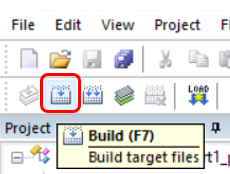
\includegraphics[width=1.5in]{figure/uv5/IDE_build_button}
      \captionof{figure}{Keil IDE: Build Target} 
      \label{fig_ide_build_button}
    \end{minipage}
If nothing goes wrong, the build output window at the bottom of the IDE will show a log similar like the one shown in Figure \ref{fig_ide_build}. \par  
    \begin{minipage}{\linewidth}
      \centering
      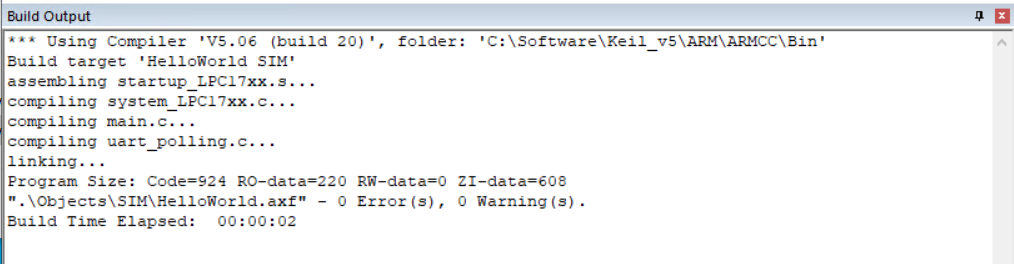
\includegraphics[width=5in]{figure/uv5/IDE_build}
      \captionof{figure}{Keil IDE: Build Target} 
      \label{fig_ide_build}
    \end{minipage}

\section{Debug the Target}
In theory, you may now load the target by pressing the LOAD button. However please {\em pause} before you attempt to do it. Our final goal is to build a project that is ready to be released and then load it to the on-chip flash to ship it to the customer. However we will need to do lots of debugging before we reach this goal. Keep flashing the board will greatly shorten the life of the on-chip memory since there is a limited number of times one can flash it. So for development purpose, developers rarely press the LOAD button in the IDE to load the image to the flash memory since each load action writes to the flash memory cells. Most of the time we use the simulator to debug and execute our project. We will also show you a commonly used technique to load the target to RAM, which has a lot longer life span than flash memory, and debug the target on the board by using the ULINK-ME hardware debugger in Section \ref{sec_debug_target_ram}.

%You can use either the simulator within the IDE or the ULINK Cortex Debugger to debug your program. To start a debug session, click Debug$\rightarrow$Start/Stop Debug Session from the IDE menu bar or press Ctrl+F5. As any other GUI debugger, the IDE allows you to set up break points and step through your source code. It also shows the registers, which is very helpful for debugging low level code. Click View, Debug and Peripherals from the IDE menu bar and explore the functionality of the debugger.

  \subsection{Debug the Project in Simulator}
    We will configure our project to use the simulator as the debugger.
    \begin{enumerate}
    \item Open up the target option window and select ``Use Simulator'' in the Debug tab and set the Dialog DLL and Parameters as shown Figure \ref{fig_ide_opt_debug_tab}.
    The debug script \verb+SIM.ini+ provided in the starter code (see Listing \ref{lst_sim_ini} in
    Appendix \ref{app_debug_ini}) is needed to map the second bank of RAM area read and write
    accessible inside the simulator. \par
      % Some versions of the uVision IDE does not set up the debugger properly for the LPC1768. Check that the Dialog DLL and Parameter settings are configured as shown in Figure \ref{fig_ide_opt_debug_tab}.
          \begin{minipage}{\linewidth}
            \centering
            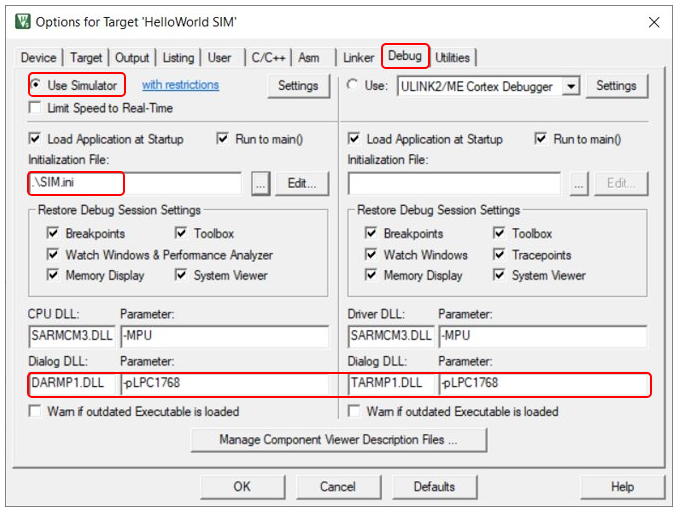
\includegraphics[width=4in]{figure/uv5/IDE_opt_debug_tab}
            \captionof{figure}{Keil IDE: Target Options Debug Tab Configuration} 
            \label{fig_ide_opt_debug_tab}
          \end{minipage}

      \item Press the ``debug'' button to bring up the debugger interface (See Figure \ref{fig_ide_debug_button}). \par
        \begin{minipage}{\linewidth}
          \centering
          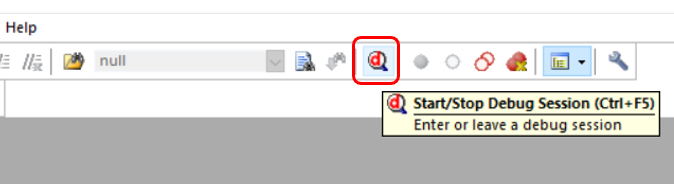
\includegraphics[width=4in]{figure/uv5/IDE_debug_button}
          \captionof{figure}{Keil IDE: Debug Button} 
          \label{fig_ide_debug_button}
        \end{minipage}

      \item Select UART1 and UART2 (see Figure \ref{fig_ide_sim_uart_button}) from the serial window drop down list so that they appear in simulator (see Figure \ref{fig_ide_sim_uart}). Note that the hardware UART index starts from 0 and the simulator UART index starts from 1. So the UART1 window in simulator is for the UART0 on the board. The UART2 window in simulator is for the UART1 on the board. \par 

        \begin{minipage}{\linewidth}
          \centering
          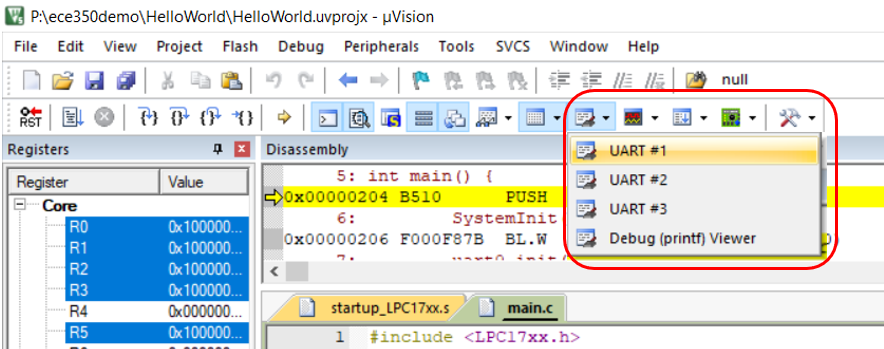
\includegraphics[width=4in]{figure/uv5/IDE_sim_uart_button}
          \captionof{figure}{Keil IDE: Debugging. Enable Serial Window View.} 
          \label{fig_ide_sim_uart_button}
        \end{minipage}
        \par
        \begin{minipage}{\linewidth}
          \centering
          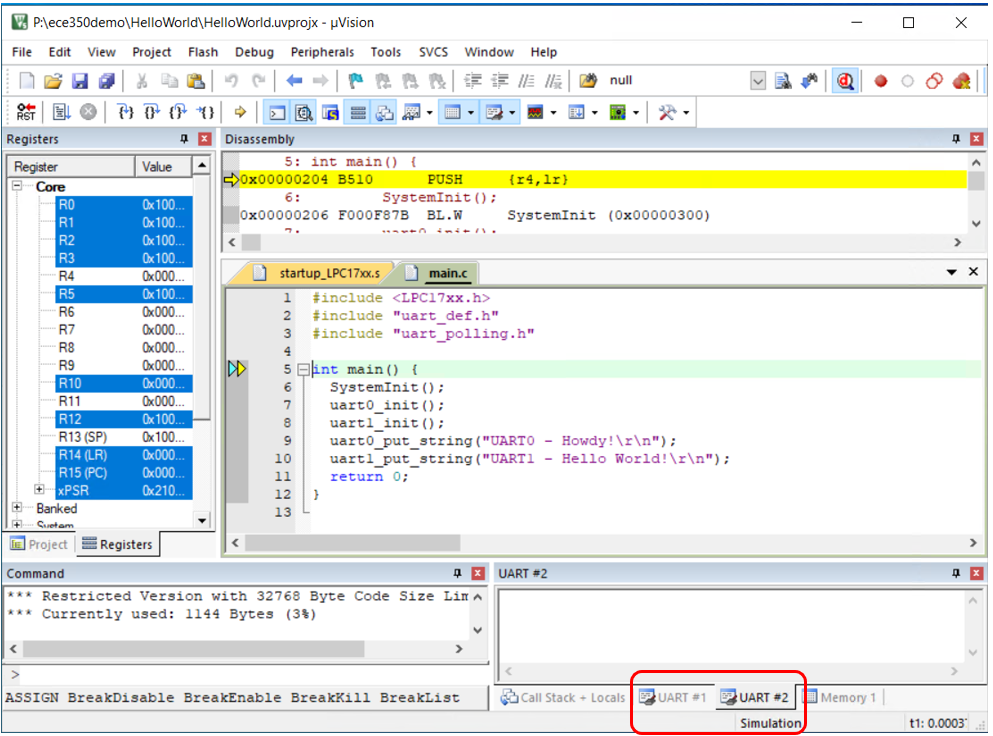
\includegraphics[width=4in]{figure/uv5/IDE_sim_uart}
          \captionof{figure}{Keil IDE: Debugging. Both UART0 and UART1 views are enabled in simulator.} 
          \label{fig_ide_sim_uart}
        \end{minipage}

      \item Press the ``Run'' button on the menu to let the program execute (see Figure \ref{fig_ide_run_button}). You will see the output of UART0 appearing in UART1 simulator window and the output of UART1 appearing in UART2 simulator window (see Figure \ref{fig_ide_output}). Note that we moved the UART windows from their default positions in the simulator for better view. \par
        \begin{minipage}{\linewidth}
          \centering
          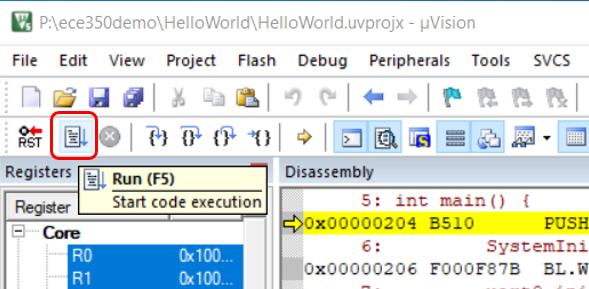
\includegraphics[width=3.5in]{figure/uv5/IDE_run_button}
          \captionof{figure}{Keil IDE: Debugging. The Run Button.} 
          \label{fig_ide_run_button}
        \end{minipage}
        \par
        \begin{minipage}{\linewidth}
          \centering
          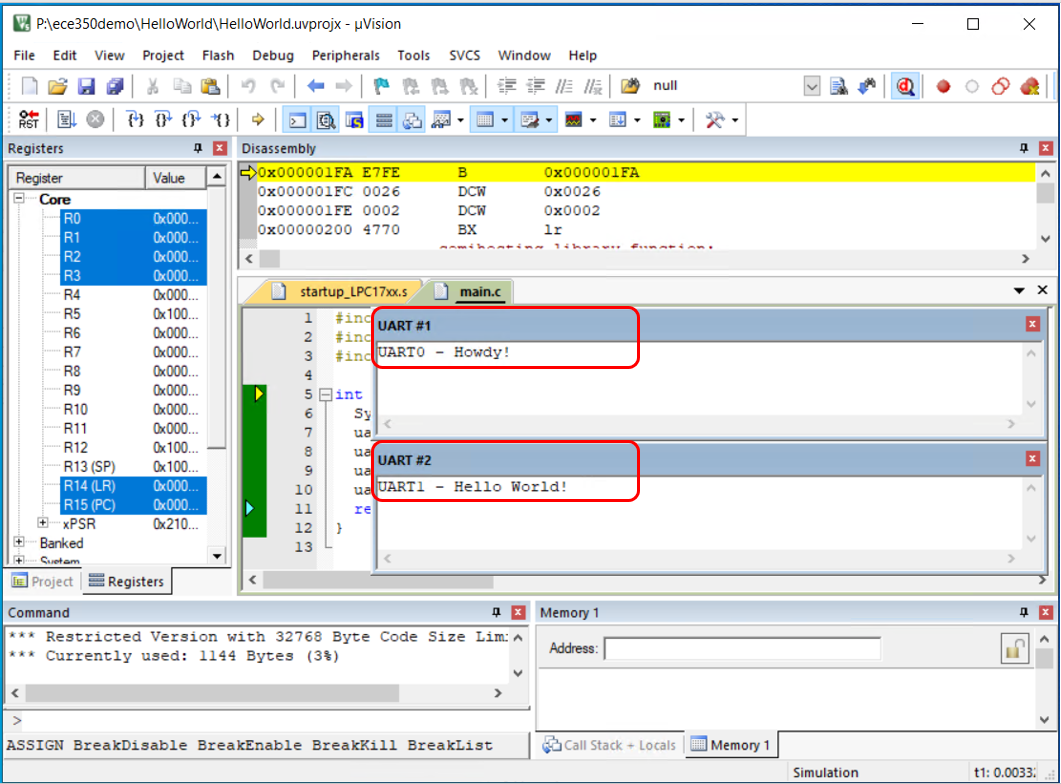
\includegraphics[width=6in]{figure/uv5/IDE_output}
          \captionof{figure}{Keil IDE: Debugging Output.} 
          \label{fig_ide_output}
        \end{minipage}

      \item To exit the debugging session, press the ``debug'' button again (see Figure \ref{fig_ide_debug_button}).

\end{enumerate}

  %\subsubsection*{Configure In-Memory Execution Using ULINK-ME Cortex Debugger}
  \subsection{Debug the Project on the Board by In-Memory Execution}
  \label{sec_debug_target_ram}
When debugging the code on the board, we use the ULINK-ME Cortex Debugger. The code will execute on the board. You will find creating a separate hardware debug target makes the development process easier. 

    \begin{enumerate}
      \item Press the Managing Project Item button (see Figure \ref{fig_ide_component_button}). \par
        \begin{minipage}{\linewidth}
            \centering
            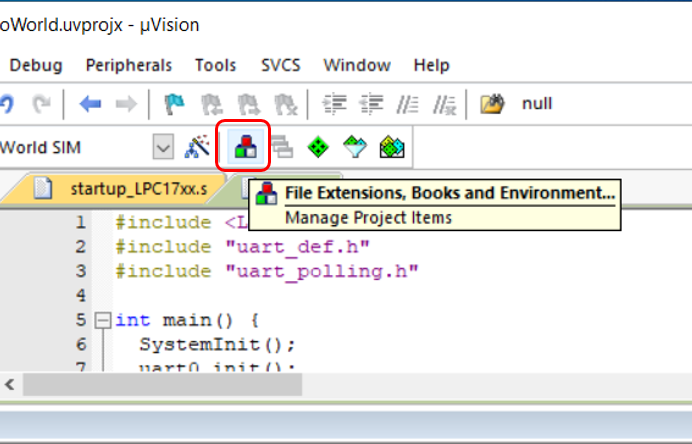
\includegraphics[width=4in]{figure/uv5/IDE_component_button}
            \captionof{figure}{Keil IDE: Manage Project Items Button} 
            %\caption{Keil IDE: Manage Project Items Button} 
            \label{fig_ide_component_button}
        \end{minipage}
  
      \item Press the New icon to create a new target and name it ``HelloWorld RAM''(see Figure \ref{fig_ide_components}). The new target duplicates the HelloWorld SIM target configuration. \par 

          \begin{minipage}{\linewidth}
            \centering
            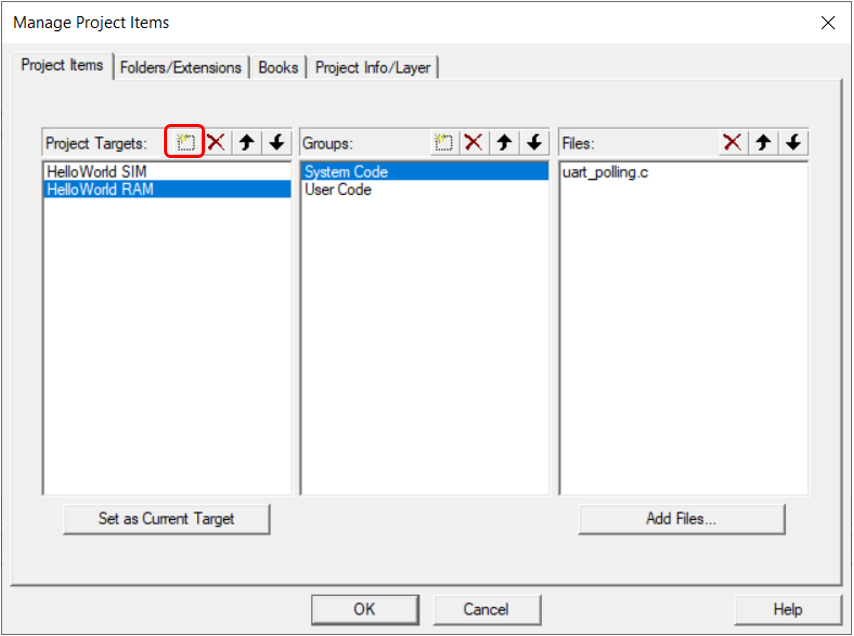
\includegraphics[width=5in]{figure/uv5/IDE_components}
            \captionof{figure}{Keil IDE: Manage Project Items Window.} 
            \label{fig_ide_components}
          \end{minipage}

        \item Switch your target to the newly created RAM target (See Figure \ref{fig_ide_target_ram}).\par

          \begin{minipage}{\linewidth}
            \centering
            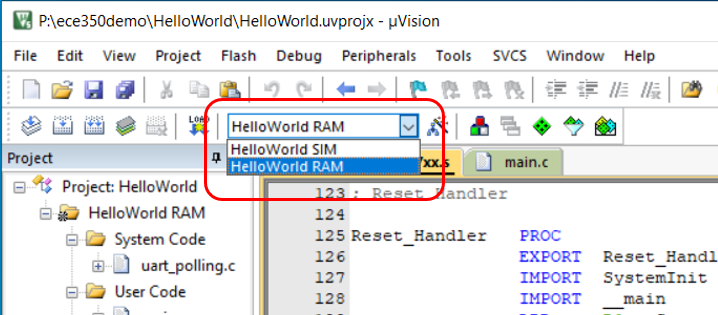
\includegraphics[width=4in]{figure/uv5/IDE_target_ram}
            \captionof{figure}{Keil IDE: Select HelloWorld RAM Target.} 
            \label{fig_ide_target_ram}
          \end{minipage}
        Configure in-memory code execution as shown in Figure \ref{fig_ide_opt_target_tab_ram}. \par
          \begin{minipage}{\linewidth}
            \centering
            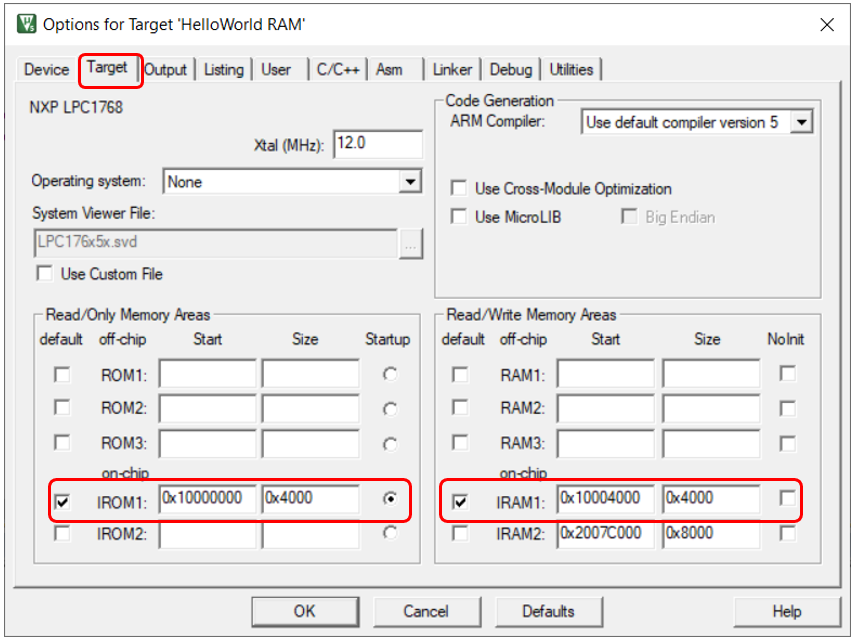
\includegraphics[width=4in]{figure/uv5/IDE_opt_target_tab_ram}
            \captionof{figure}{Keil IDE: Configure Target Options Target Tab for In-memory Execution.} 
            \label{fig_ide_opt_target_tab_ram}
          \end{minipage}

        The default image memory map setting is that the code is executed from the ROM (see Figure \ref{fig_ide_opt_target_tab}). Since the ROM portion of the code needs to be flashed in order to be executed on the board, this incurs wear-and-tear on the on-chip flash of the LPC1768. Since most attempts to write a functioning RTX will eventually require some more or less elaborate debugging, the flash memory might wear out quickly. Unlike the flash memory stick file systems where the wear is aimed to be uniformly distributed across the memory portion, this flash memory will get used over and over again in the same portion.

        The ARM compiler can be configured to have a different starting address. The configuration in Figure \ref{fig_ide_opt_target_tab_ram} makes code starting address in RAM.

        \item Select the Asm tab and input \verb+NO_CRP+ in the Conditional Assembly Control Symbols section as shown in Figure \ref{fig_ide_asm_no_crp}. \par

          \begin{minipage}{\linewidth}
            \centering
            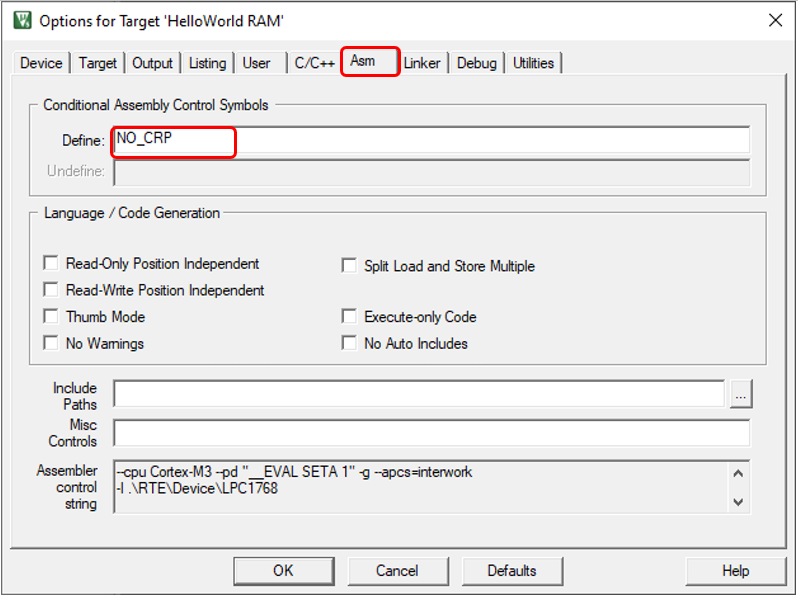
\includegraphics[width=5in]{figure/uv5/IDE_asm_no_crp}
            \captionof{figure}{Keil IDE: RAM Target Asm Configuration.} 
            \label{fig_ide_asm_no_crp}
          \end{minipage}

        \item Select the ULINK2/ME Cortex Debugger in the target options Debug tab and use an debug script \verb+RAM.ini+ provided in the starter code (See Figure \ref{fig_ide_opt_debug_tab_ulink}) as a initialization file.
An initialization file \verb+RAM.ini+ (see Listing \ref{lst_ram_ini} in Appendix \ref{app_debug_ini}) is needed to do the proper setting of SP, PC and vector table offset register. \par

          \begin{minipage}{\linewidth}
            \centering
            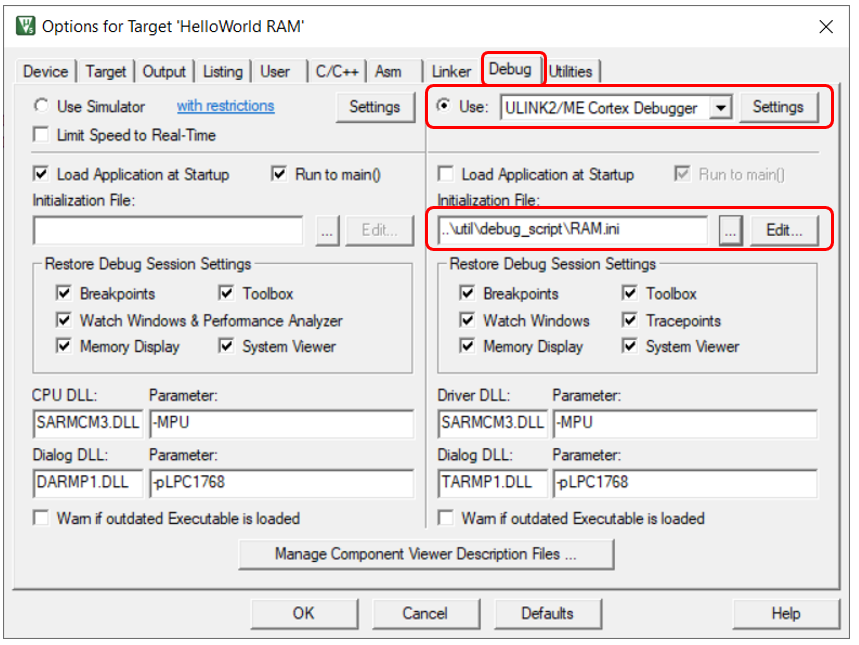
\includegraphics[width=4in]{figure/uv5/IDE_opt_debug_tab_ulink}
            \captionof{figure}{Keil IDE: Configure ULINK-ME Hardware Debugger.} 
            \label{fig_ide_opt_debug_tab_ulink}
          \end{minipage}

        \item Press the settings button beside the ULINK2/ME Cortex Debugger (see Figure \ref{fig_ide_opt_debug_tab_ulink}) and select the Flash Download tab (see Figure \ref{fig_ide_flash_algo_empty}). Remove the LPC17xx IAP 512kB Flash algorithm to the Programming Algorithm field if it is there. \par
  
          \begin{minipage}{\linewidth}
            \centering
            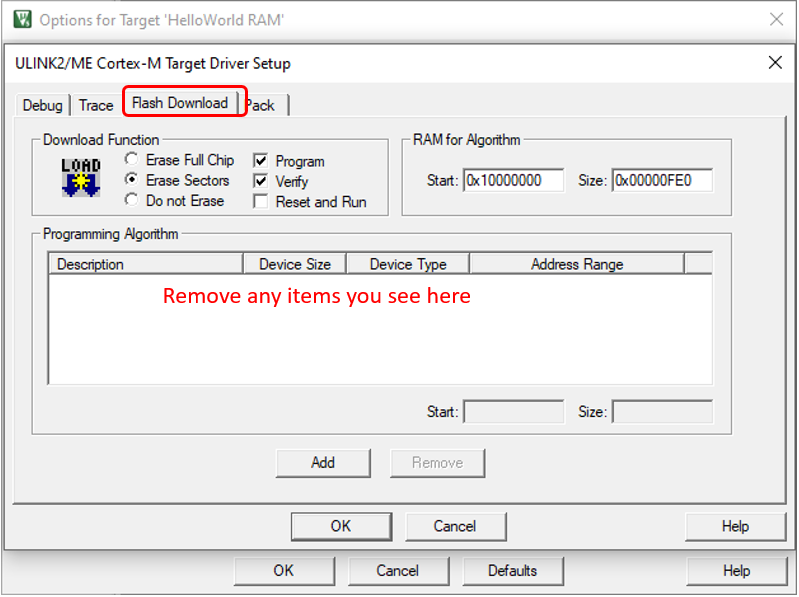
\includegraphics[width=5in]{figure/uv5/IDE_flash_algo_empty}
            \captionof{figure}{Keil IDE: Flash Download Programming Algorithm Configuration.} 
            \label{fig_ide_flash_algo_empty}
          \end{minipage}

        \item Select the Utilities tab and select the radio button beside ``Use External Tool for Flash Programming'' (see Figure \ref{fig_ide_utilities_ram_target}).\par  

          \begin{minipage}{\linewidth}
            \centering
            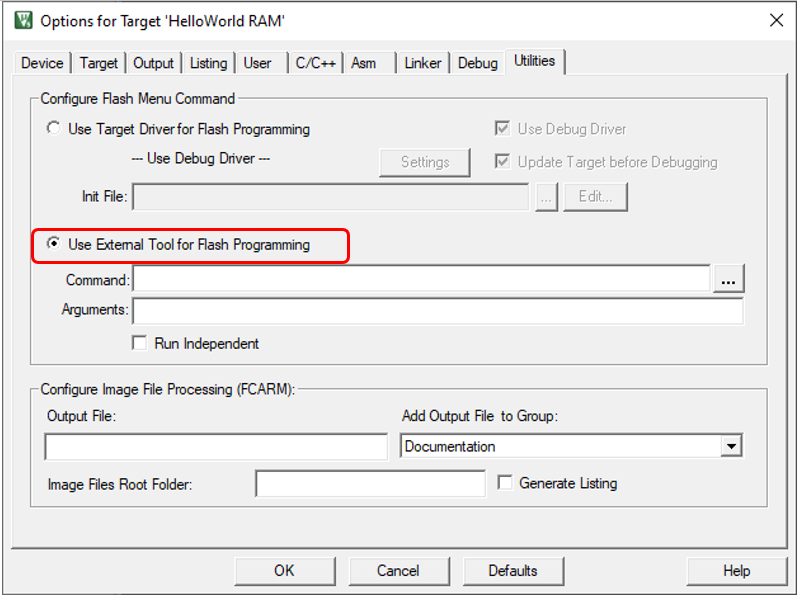
\includegraphics[width=4in]{figure/uv5/IDE_utilities_ram_target}
            \captionof{figure}{Keil IDE: Target Option Utilities Configuration for RAM Target.} 
            \label{fig_ide_utilities_ram_target}
          \end{minipage}

        \item Open the PuTTY terminals to see the output. You will need a terminal emulator such as PuTTY that talks directly to COM ports in order to see output of the serial port. To find out the two COM ports, open up the device manager and expand the Ports (COM \& LPT) line (see Figure \ref{fig_device_manager_ports}). \par

          \begin{minipage}{\linewidth}
            \centering
            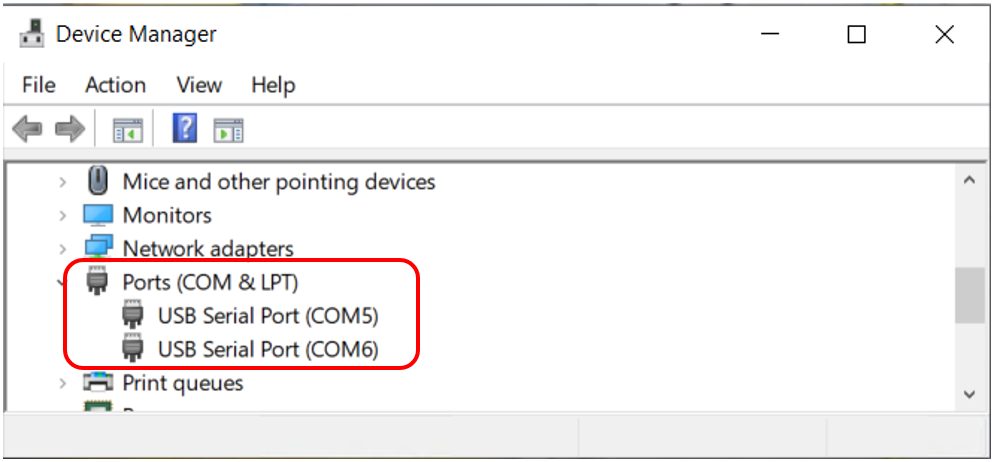
\includegraphics[width=4in]{figure/device_manager_ports_rc}
            \captionof{figure}{Device Manger COM Ports} 
            \label{fig_device_manager_ports}
          \end{minipage}
          Note the COM port numbers are different for each lab computer. The COM port numbers may also change after a reboot of the computer.
  An example PuTTY Serial configuration is shown in Figures \ref{fig_putty_uart_session} and \ref{fig_putty_uart_config}.

          \begin{minipage}{\linewidth}
            \centering
            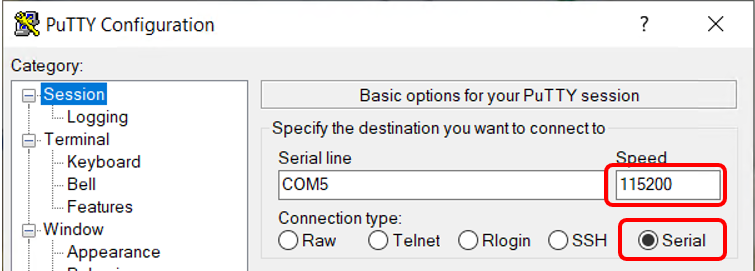
\includegraphics[width=4in]{figure/putty_uart_session_rc}
            \captionof{figure}{PuTTY Session for Serial Port Communication} 
            \label{fig_putty_uart_session}
          \end{minipage}
          \par
          \begin{minipage}{\linewidth}
            \centering
            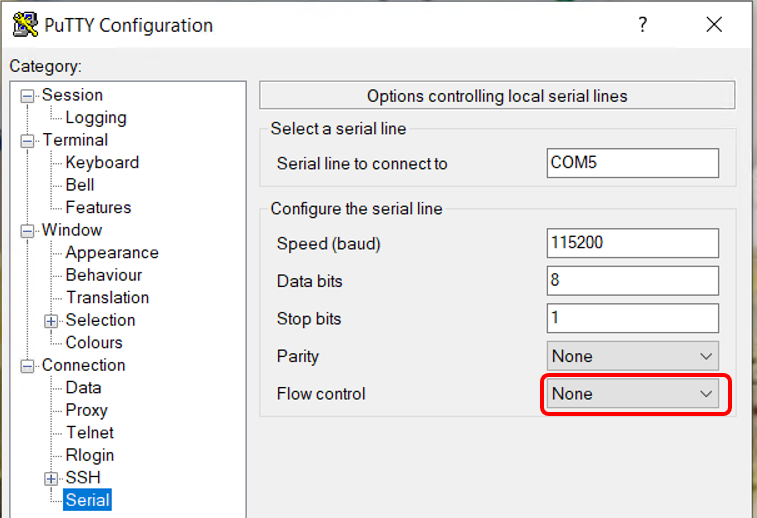
\includegraphics[width=4in]{figure/putty_uart_config_rc}
            \captionof{figure}{PuTTY Serial Port Configuration} 
            \label{fig_putty_uart_config}
          \end{minipage}
 
        \item To download the code to the board, {\em do not press the LOAD button}. Instead, the {\em debug button} is pressed to initiate a debug session and the \verb+RAM.ini+ file will load the code to the board.
        \item Either step through the code or just press the Run button to execute the code till the end. You will see output from your PuTTY terminals (see Figure \ref{fig_putty_output_helloworld}).

          \begin{minipage}{\linewidth}
            \centering
            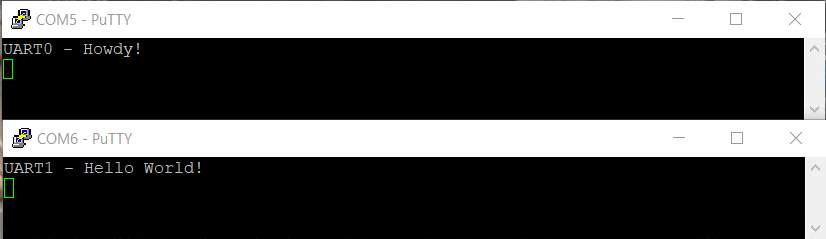
\includegraphics[width=5in]{figure/putty_out_helloworld}
            \captionof{figure}{PuTTY Output} 
            \label{fig_putty_output_helloworld}
          \end{minipage}
      \end{enumerate}
\section{Download to ROM}
Though we keep discouraging you to download the image to ROM, we walk you through the steps on how to do it to give you a feel of how a project that is ready to be released is loaded to the ROM. We expect that you already fixed your code by debugging the code on board by using the in-memory execution technique we showed you earlier. You should only do the following experiment once or twice. Please use the ROM sparingly.

Switch your target to the ``HelloWorld SIM'' target (see Figure \ref{fig_ide_load_button}). Open up the target option. Select the Debug tab and press the ``Settings'' button beside the ULINK2/ME Debugger (upper right portion of the window). Select the ``Flash Download'' tab and check the box ``Reset and Run'' in the Download Function section (See Figure \ref{fig_ide_flash_algo_reset_run}). This will execute the code automatically without the need to press the physical reset button on the board. Add the LPC17xx IAP 512kB Flash algorithm to the Programming Algorithm field if it is not already there. Apply all the changes and close the target options configuration window. \par

  \begin{minipage}{\linewidth}
    \centering
    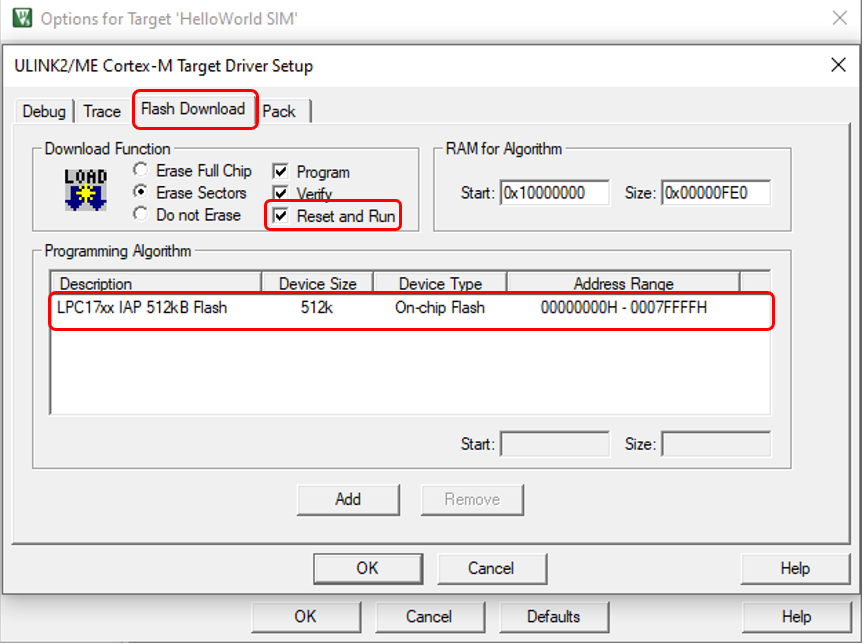
\includegraphics[width=4.5in]{figure/uv5/IDE_flash_algo_reset_run}
    \captionof{figure}{Flash Download Reset and Run Setting} 
    \label{fig_ide_flash_algo_reset_run}
  \end{minipage} \\

To download the code to the on-chip ROM, click the ``Load" button (see Figure \ref{fig_ide_load_button}). 
The download is through the ULINK-ME. The code automatically runs. You should see the output from PuTTY terminals.\par
  \begin{minipage}{\linewidth}
    \centering
    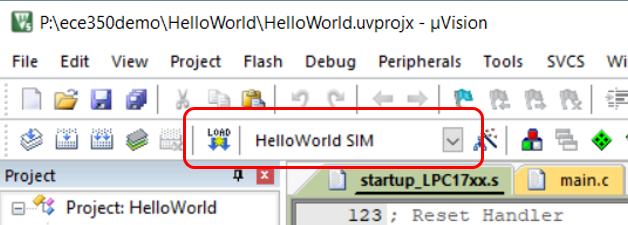
\includegraphics[width=3.5in]{figure/uv5/IDE_load_button}
    \captionof{figure}{Keil IDE: Download Target to Flash} 
    \label{fig_ide_load_button}
  \end{minipage}

%(\begin{wrapfigure}{r}{4mm}
% \centering
% \includegraphics[height=3mm]{figure/IDE_load_icon}
% \end{wrapfigure}
%). 
